\documentclass{article}
\usepackage{amsmath}
\usepackage{amssymb}
\usepackage[a4paper, top=25mm, bottom=25mm, left=25mm, right=25mm]{geometry}
\usepackage{pgfplots}
\usepackage{cancel}
\usepackage{mathtools}
\pgfplotsset{compat=1.18}
\usepgfplotslibrary{polar}
\usepgfplotslibrary{fillbetween}
\usepackage{tikz}
\usetikzlibrary{arrows.meta}

\begin{document}
\pagestyle{empty}
\large

\begin{center}
2019-2020 Spring \\MAT124-02,05 Final\\(01/07/2020)
\end{center}

\noindent 1. Find the maximum and minimum values of the function $f(x,y,z)=x-y+z$ on the sphere $x^2+y^2+z^2=100$.

\hfill

\noindent 2. A cylindrical tank is $4$ ft high and has an outer diameter of $2$ ft. The walls of the tank are $0.2$ in. thick. Approximate the volume of the interior of the tank assuming the tank has a top and bottom that are both also $0.2$ in. thick.

\hfill

\noindent 3. Let $z=f(x,y)$ be a differentiable function of $x$ and $y$, and let $x=r\cos\theta$ and $y=r\sin\theta$ for $r>0$ and $0<\theta<2\pi$. Show that

\[\left(\frac{\partial z}{\partial r}\right)^2+\frac1{r^2}\left(\frac{\partial z}{\partial\theta}\right)^2=\left(\frac{\partial z}{\partial x}\right)^2+\left(\frac{\partial z}{\partial y}\right)^2.\]

\hfill

\noindent 4. Reverse the order of integration in

\[\displaystyle\int_1^2\int_x^{x^3}f(x,y)\,dy\,dx+\int_2^8\int_x^8f(x,y)\,dy\,dx.\]

\hfill

\noindent 5. Evaluate the double integral

\[\int_1^2\int_{y^2}^{y^5}\mathrm{e}^{x/y^2}\,\xcancel{dy\,dx}\,dx\,dy.\]

\hfill

\noindent 6. Use a double integral to find the area of the region that lies inside the circle $r=\cos\theta$ and outside the cardioid $r=1-\cos\theta$.

\hfill

\noindent 7. Evaluate the volume of the solid bounded below by the cone $z=\sqrt{x^2+y^2}$ and above by the paraboloid $z=2-x^2-y^2$, by using a triple integral in cylindrical coordinates.

\hfill

\noindent 8. Let $T$ be the solid in the first octant bounded above by the sphere $x^2+y^2+z^2=7$ and below by the paraboloid $z=x^2+y^2$. Express (do not evalaute) the integral

\[\iiint_T\sin\left(\sqrt{x^2+y^2+z^2}\right)\,dV\]

\hfill

\noindent in spherical coordinates.

\newpage

\begin{center}
2019-2020 Spring Final (01/07/2020) Solutions\\
(Last update: 8/5/25 (8th of August) 10:40 PM)
\end{center}

\noindent 1. Let $g(x,y,z)=x^2+y^2+z^2-100$ and then, solve the system of equations below using the method of Lagrange multipliers.

\[
\left.
\begin{array}{l}
\displaystyle\nabla f=\lambda\nabla g\\
\displaystyle g(x,y,z)=0
\end{array}
\right\}\quad\begin{array}{c}
\nabla f=\left\langle1,-1,1\right\rangle=\lambda\left\langle2x,2y,2z\right\rangle=\lambda\nabla g\\[1em]\displaystyle\therefore\: x=\frac1{2\lambda},\quad y=-\frac1{2\lambda},\quad z=\frac1{2\lambda}
\end{array}
\]

\hfill

\noindent Use the constraint.

\[g(x,y,z)=0\implies\left(\frac1{2\lambda}\right)^2+\left(-\frac1{2\lambda}\right)^2+\left(\frac1{2\lambda}\right)^2=100\implies\frac3{4\lambda^2}=100\implies\lambda=\pm\frac{\sqrt3}{20}\]

\[\lambda=\pm\frac{\sqrt3}{20\lambda}\implies x=\pm\frac{10\sqrt3}3,\quad y=\mp\frac{10\sqrt3}3,\quad z=\pm\frac{10\sqrt3}3\quad\]

\hfill

\noindent The absolute extrema occur at $\left(\frac{10\sqrt3}3,-\frac{10\sqrt3}3,\frac{10\sqrt3}3\right)$ and $\left(-\frac{10\sqrt3}3,\frac{10\sqrt3}3,-\frac{10\sqrt3}3\right)$.

\[f\left(\frac{10\sqrt3}3,-\frac{10\sqrt3}3,\frac{10\sqrt3}3\right)=10\sqrt3,\quad f\left(-\frac{10\sqrt3}3,\frac{10\sqrt3}3,-\frac{10\sqrt3}3\right)=-10\sqrt3\]

\[\boxed{\text{The minimum value is }{-10\sqrt3}\text{ and the maximum value is }10\sqrt3.}\]

\hfill

\noindent 2. Recall that 12 inches is 1 foot. The volume of a right circular cylinder is

\[V(r,h)=\pi r^2 h\]

\hfill

\noindent The total differential is

\[dV=V_r\,dr+V_h\,dh=\pi\left(2r\cdot h\right)\,dr+\pi\left(r^2\cdot 1\right)\,dh\]

\hfill

\noindent Set $r=1,\:h=4,\:dr=-0.2/12=-1/60,\:dh=-0.4/12=-1/30$.

\[dV=\pi\left(2\cdot1\cdot 4\right)\cdot\left(-\frac1{60}\right)+\pi\left(1^2\right)\left(-\frac1{30}\right)=-\frac\pi6\]

\hfill

\noindent Calculate the volume of the outer cylinder.

\[V(1,4)=\pi\cdot1^2\cdot4=4\pi\]

\hfill

\noindent Take $\displaystyle\Delta V\approx dV=-\frac\pi6$. Therefore, the volume of the interior can be approximated as follows.

\[\boxed{V\approx4\pi-\frac\pi6=\frac{23\pi}6}\]

\newpage

\noindent 3. We have $x=r\cos\theta$ and $y=r\sin\theta$. Compute the first-order partial derivatives.

\[\frac{\partial z}{\partial r}=\frac{\partial z}{\partial x}\cdot\frac{\partial x}{\partial r}+\frac{\partial z}{\partial y}\cdot\frac{\partial y}{\partial r},\qquad\frac{\partial z}{\partial \theta}=\frac{\partial z}{\partial x}\cdot\frac{\partial x}{\partial \theta}+\frac{\partial z}{\partial y}\cdot\frac{\partial y}{\partial \theta}\]

\hfill

\[\frac{\partial x}{\partial r}=\cos\theta,\qquad\frac{\partial y}{\partial r}=\sin\theta,\qquad\frac{\partial x}{\partial \theta}=-r\sin\theta,\qquad\frac{\partial y}{\partial\theta}=r\cos\theta,\]

\hfill

\noindent Rewrite $\displaystyle\frac{\partial z}{\partial r}$ and $\displaystyle\frac{\partial z}{\partial\theta}$.

\[\frac{\partial z}{\partial r}=\frac{\partial z}{\partial x}\cdot\cos\theta+\frac{\partial z}{\partial y}\cdot\sin\theta\]

\[\frac{\partial z}{\partial\theta}=\frac{\partial z}{\partial x}\cdot(-r\sin\theta)+\frac{\partial z}{\partial y}\cdot(r\cos\theta)\implies\frac1r\cdot\frac{\partial z}{\partial\theta}=\frac{\partial z}{\partial x}\cdot(-\sin\theta)+\frac{\partial z}{\partial y}\cdot\cos\theta\]

\hfill

\noindent Take the squares of both sides of the equations and add up side by side.

\[\left(\frac{\partial z}{\partial r}\right)^2=\left(\frac{\partial z}{\partial x}\cdot\cos\theta+\frac{\partial z}{\partial y}\cdot\sin\theta\right)^2,\quad\left(\frac1r\cdot\frac{\partial z}{\partial\theta}\right)^2=\left(\frac{\partial z}{\partial x}\cdot(-\sin\theta)+\frac{\partial z}{\partial y}\cdot\cos\theta\right)^2\]

\hfill

\begin{align*}
\left(\frac{\partial z}{\partial r}\right)^2+\frac1{r^2}\left(\frac{\partial z}{\partial\theta}\right)^2&=\left(\frac{\partial z}{\partial x}\right)^2\cos^2\theta+\frac{\partial z}{\partial x}\cdot\frac{\partial z}{\partial y}\cdot\cos\theta\sin\theta+\left(\frac{\partial z}{\partial y}\right)^2\sin^2\theta\\\\&\quad\:\;+\left(\frac{\partial z}{\partial x}\right)^2\sin^2\theta-\frac{\partial z}{\partial x}\cdot\frac{\partial z}{\partial y}\cdot\cos\theta\sin\theta+\left(\frac{\partial z}{\partial y}\right)^2\cos^2\theta
\end{align*}

\hfill

\noindent The terms with $\sin\theta\cos\theta$ cancel each other. Recall the equation $\displaystyle \sin^2x+\cos^2x=1$. The equation then becomes

\[\left(\frac{\partial z}{\partial r}\right)^2+\frac1{r^2}\left(\frac{\partial z}{\partial\theta}\right)^2=\left(\frac{\partial z}{\partial x}\right)^2+\left(\frac{\partial z}{\partial y}\right)^2,\]

\hfill

\noindent which we set out to demonstrate.

\hfill

\noindent 4.
\begin{center}
\begin{minipage}{0.5\textwidth}
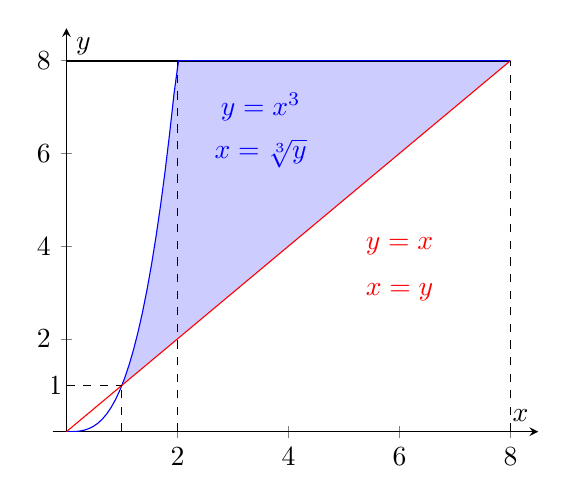
\begin{tikzpicture}
  \begin{axis}[
      axis lines = middle,
      xlabel = $x$, ylabel = $y$,
      domain=0:8,
      ymin=0, ymax=8.7,
      xmin=-0.25, xmax=8.5,
      samples=100,
      clip=true,
      scale=0.9,
    ]
    
    \addplot [name path=A, domain=1:8, draw=none] {x};
    \addplot [name path=B, domain=1:8, draw=none] {min(x^3,8)};
    \addplot [fill=blue!20, draw=none] fill between [of=A and B, soft clip={domain=1:8}];

    \node at (-0.2,1) {$1$};
    \draw[thick] (0,8)--(8,8);
    \addplot [blue, domain=0:8] {min(x^3,8)};
    \addplot [red, domain=0:8] {x};
    \draw[dashed] (1,0)--(1,1); \draw[dashed] (0,1)--(1,1); \draw[dashed] (2,0)--(2,8); \draw[dashed] (8,0)--(8,8);

    \node[red] at (6,4) {$y=x$}; \node[red] at (6,3) {$x=y$};
    \node[blue] at (3.5,7) {$y=x^3$}; \node[blue] at (3.5,6) {$x=\sqrt[3]{y}$};
  \end{axis}
\end{tikzpicture}
\end{minipage}\begin{minipage}{0.45\textwidth}
\[\boxed{\int_1^8\int_{\sqrt[3]y}^yf(x,y)\,dx\,dy}\]
\end{minipage}
\end{center}

\newpage

\noindent 5. \textbf{Remark}: There was a mistake in the original question. The order of integration must be reversed.

\begin{align*}\int_1^2\int_{y^2}^{y^5}\mathrm{e}^{x/y^2}\,dx\,dy&=\int_1^2\left[y^2\cdot{\mathrm{e}^{x/y^2}}\right]_{x=y^2}^{x=y^5}\,dy=\int_1^2\left(y^2\cdot\mathrm{e}^{y^3}-y^2\cdot\mathrm{e}\right)\,dy=\left[\frac13\mathrm{e}^{y^3}-\frac13\mathrm{e}y^3\right]_1^2\\\\&=\frac13\mathrm{e}^{8}-\frac{8\mathrm{e}}3-\left(\frac13\mathrm{e}^1-\frac13\mathrm{e}\right)=\boxed{\frac{\mathrm{e}}3\left(\mathrm{e}^7-8\right)}\end{align*}

\hfill

\noindent 6.
\begin{center}
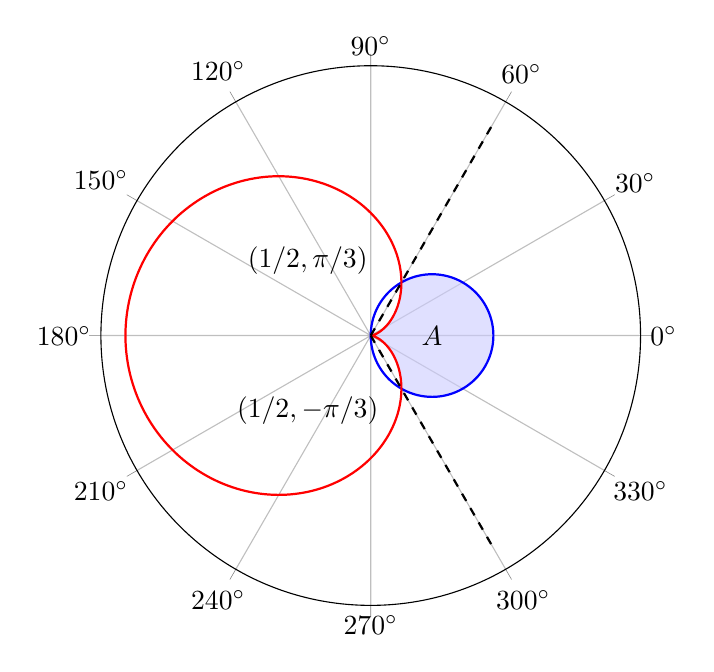
\begin{tikzpicture}
  \begin{polaraxis}[ytick=\empty, axis y line=none, xticklabel=$\pgfmathprintnumber{\tick}^\circ$,]
    \addplot [
      domain=-pi/3:pi/3,
      samples=300,
      draw=none,
      name path=A,
      data cs=polarrad,
    ] {cos(deg(x))};

    \addplot [
      domain=-pi/3:pi/3,
      samples=300,
      draw=none,
      name path=B,
      data cs=polarrad,
    ] {1-cos(deg(x))};

    \addplot [
      blue!20,
      fill opacity=0.6,
    ] fill between[of=A and B];

    \addplot [
      domain=0:2*pi,
      samples=300,
      thick,
      blue,
      data cs=polarrad,
    ] {cos(deg(x))};

    \addplot [
      domain=0:2*pi,
      samples=300,
      thick,
      red,
      data cs=polarrad,
    ] {1-cos(deg(x))};

    \draw[black, thick, dashed] (axis cs: 60,0) -- (axis cs: 60,2);
    \draw[black, thick, dashed] (axis cs: -60,0) -- (axis cs: -60,2);

    \node at (axis cs:130,0.8) {$(1/2,\pi/3)$};
    \node at (axis cs:-130,0.8) {$(1/2,-\pi/3)$};
    \node at (0,0.5) {$A$};

  \end{polaraxis}
\end{tikzpicture}
\end{center}

\begin{align*}
A&=\int_{-\pi/3}^{\pi/3}\int_{1-\cos\theta}^{\cos\theta}\,r\,dr\,d\theta=\frac12\int_{-\pi/3}^{\pi/3}\left[\cos^2\theta-(1-\cos\theta)^2\right]\,d\theta=\frac12\int_{-\pi/3}^{\pi/3}\left(2\cos\theta-1\right)\,d\theta\\\\&=\frac12\bigg[2\sin\theta-\theta\bigg]_{-\pi/3}^{\pi/3}=\frac12\left[\left(2\sin\frac\pi3-\frac\pi3\right)-\left(2\sin\left(-\frac\pi3\right)+\frac\pi3\right)\right]=\boxed{\sqrt3-\frac\pi3}
\end{align*}

\hfill

\noindent 7. For cylindrical coordinates, we have

\[
\begin{array}{c}
z=z\\
r^2=x^2+y^2\\
dV=r\,dz\,dr\,d\theta
\end{array}\quad\rightarrow\quad
\begin{array}{c}
\displaystyle z=\sqrt{x^2+y^2}\implies z=\sqrt{r^2}\implies z_{\text{lower}}=r\\[1em]
z=2-x^2-y^2\implies z_{\text{upper}}=2-r^2\\[1em]
0\leq\theta\leq2\pi
\end{array}
\]

\hfill

\noindent Find where the surfaces $z=r$ and $z=2-r^2$ intersect to determine the upper bound of $r$.

\begin{align*}\left.\begin{array}{c}
z=r\\
z=2-r^2
\end{array}\right\}\quad r^2+r-2=0\implies (r+2)(r-1)=0\implies r_{\text{upper}}=1\end{align*}

\newpage

\begin{align*}\mathrm{I}&=\int_0^{2\pi}\int_0^1\int_{r}^{2-r^2}r\,dz\,dr\,d\theta=\int_0^{2\pi}\int_0^1\bigg[z\bigg]_{z=r}^{z=2-r^2}r\,dr\,d\theta=\int_0^{2\pi}\int_0^1\left(2-r^2-r\right)\,r\,dr\,d\theta\\\\&=\int_0^{2\pi}\int_0^1\left(2r-r^3-r^2\right)\,dr\,d\theta=\int_0^{2\pi}\left[r^2-\frac{r^4}4-\frac{r^3}3\right]_{r=0}^{r=1}\,d\theta=\int_0^{2\pi}\frac5{12}\,d\theta=\frac5{12}\cdot\theta\,\bigg|_0^{2\pi}\\\\&=\boxed{\frac{5\pi}6}\end{align*}

\hfill

\noindent 8. For spherical coordinates, we have

\[
\left.\begin{array}{c}
z=\rho\cos\phi\\
r=\rho\sin\phi\\
x^2+y^2+z^2=\rho^2\\
dV=\rho^2\sin\phi\,d\rho\,d\phi\,d\theta
\end{array}\right.\begin{array}{c}
x^2+y^2+z^2=7\implies\rho^2=7\implies\rho_{\text{upper},1}=\sqrt7\\
z=x^2+y^2\implies\rho\cos\phi=\rho^2\sin^2\phi\implies\rho_{\text{upper},2}=\cot\phi\csc\phi\\[1em]
\sin\left(\sqrt{x^2+y^2+z^2}\right)=\sin\left(\sqrt{\rho^2}\right)=\sin\rho\\[1em]
\displaystyle0\leq\theta\leq\frac\pi2
\end{array}\]

\hfill

\noindent Find where the surfaces $z=x^2+y^2$ and $x^2+y^2+z^2=7$ intersect to find the bounds of $\phi$.

\[\begin{array}{c}\displaystyle z^2+z-7=0\implies z_{1,2}=\frac{-1\pm\sqrt{1^2-4\cdot1\cdot(-7)}}2\\[1em]\displaystyle z>0\implies z=\rho\cos\phi=\sqrt7\cos\phi=\frac{-1+\sqrt{29}}{2}\\[1em]\displaystyle\cos\phi=\frac{-1+\sqrt{29}}{2\sqrt7}\implies\phi=\arccos\left(\frac{-1+\sqrt{29}}{2\sqrt7}\right)\end{array}\]

\hfill

\noindent For $\displaystyle\phi<\arccos\left(\frac{-1+\sqrt{29}}{2\sqrt7}\right)$, the upper bound for $\rho$ is $\sqrt7$. For $\displaystyle\phi>\arccos\left(\frac{-1+\sqrt{29}}{2\sqrt7}\right)$, the lower bound is $\cot\phi\csc\phi$.

\[\boxed{\begin{array}{l}\displaystyle\int_0^{\pi/2}\int_0^{\arccos\left(\textstyle\frac{-1+\sqrt{29}}{2\sqrt7}\right)}\int_0^{\sqrt7}\sin\rho \cdot\rho^2\sin\phi\,d\rho\,d\phi\,d\theta\\\\\displaystyle+\int_0^{\pi/2}\int_{\arccos\left(\textstyle\frac{-1+\sqrt{29}}{2\sqrt7}\right)}^{\pi/2}\int_0^{\cot\phi\csc\phi}\sin\rho\cdot\rho^2\sin\phi\,d\rho\,d\phi\,d\theta\end{array}}\]

\hfill

\noindent Since we choose the minimum of the upper bounds of $\rho$, we can write the equivalent expression.

\[\boxed{\int_0^{\pi/2}\int_0^{\pi/2}\int_0^{\min\left(\sqrt7,\cot\phi\csc\phi\right)}\sin\rho\cdot\rho^2\sin\phi\,d\rho\,d\phi\,d\theta}\]

\end{document}